\documentclass[12pt]{article}

%packages
\usepackage{graphicx}
\usepackage{amsmath}
\usepackage{mathdots}
\usepackage{amsthm}
\usepackage{amssymb}
\usepackage{fancyhdr}
\pagenumbering{arabic}
\usepackage{hyperref}
\usepackage{lscape}
%Margins etc...
\setlength{\textheight}{240mm}
\setlength{\topmargin}{-17mm} \setlength{\oddsidemargin}{-4mm}
\setlength{\textwidth}{166mm} \setlength{\parindent}{0mm}
\setlength{\marginparsep}{9mm} \setlength{\parskip}{3mm}

\begin{document}
\begin{center}
\Huge{Decision Tree Analysis using Precision Tree}\\
\tiny{Last updated: \today.}
\end{center}
In this lab session we will learn to use software to build decision trees. We will create the decision tree for the following situation:\\

\emph{``You are offered the opportunity of flipping a coin. If you choose to not flip you get a reward of �4 thousand. If you flip and the coin falls on \emph{heads} you get a reward of �10 thousand. If you flip and the coin falls on \emph{tails} you get nothing.''}


\begin{center}
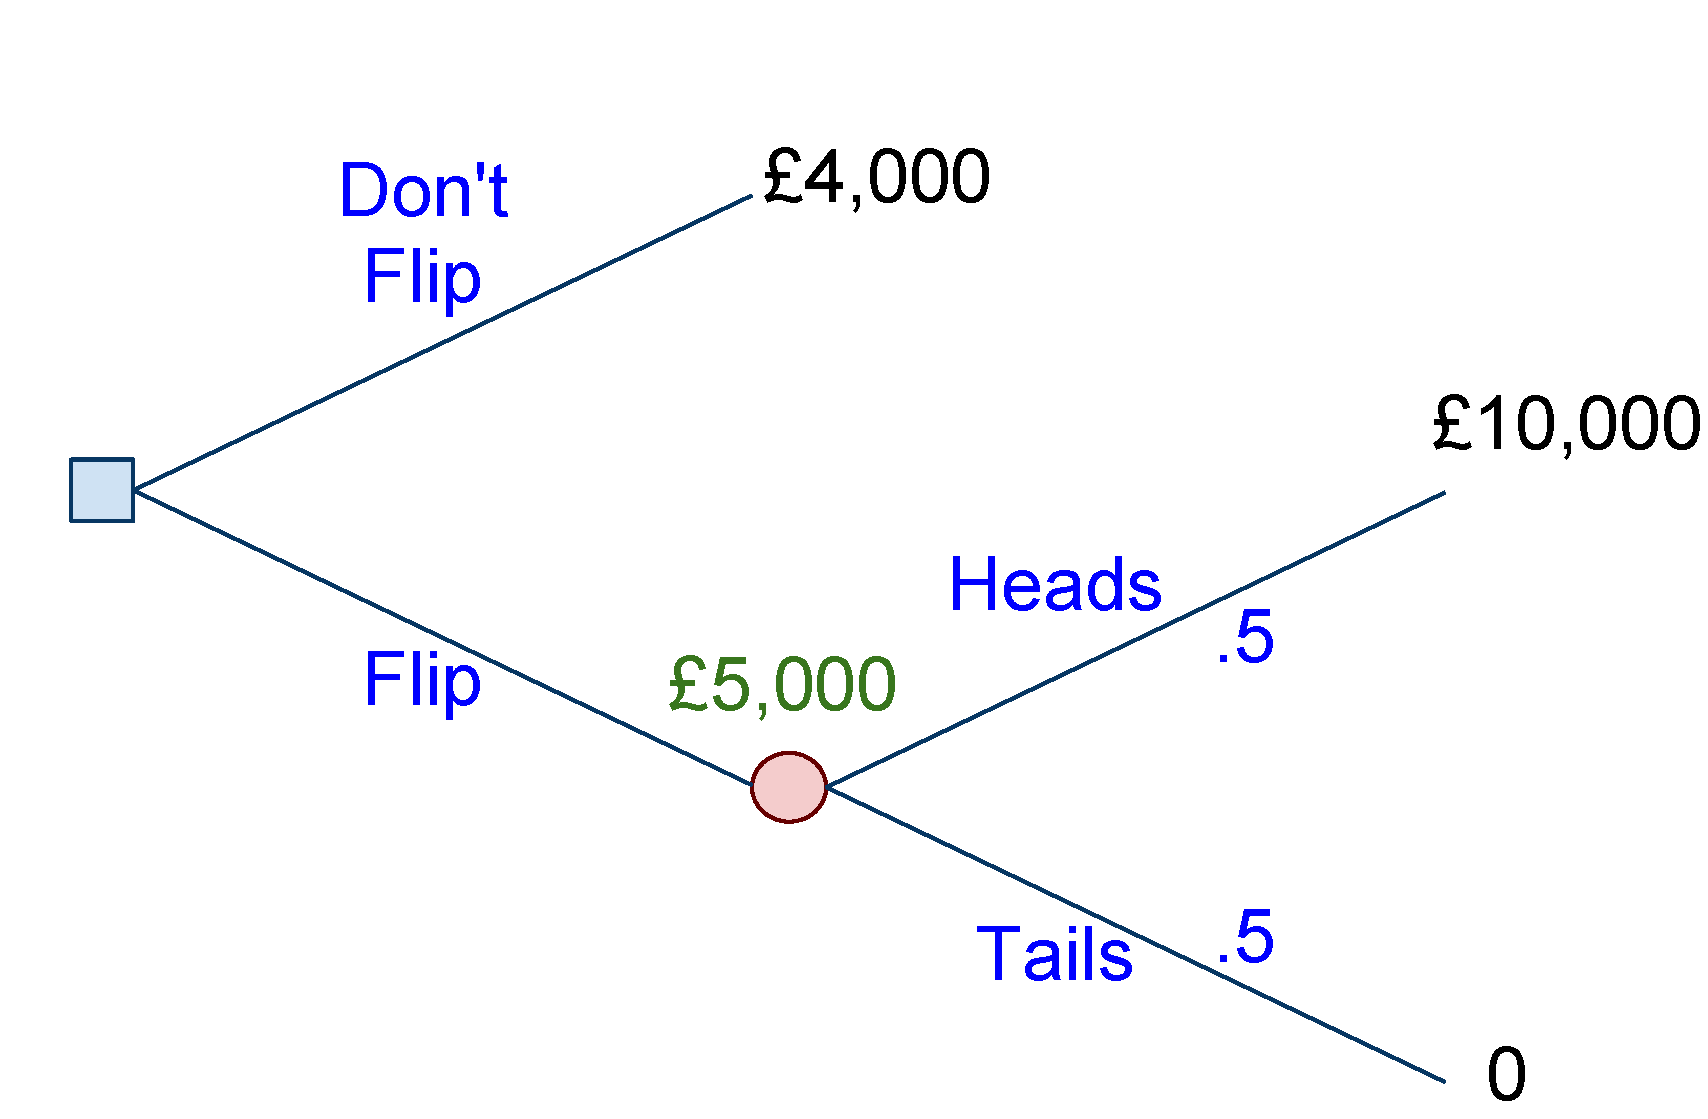
\includegraphics[width=7cm]{Coin_Flip_for_PT.pdf}
\end{center}

Steps:
\begin{itemize}
\item Build the tree:
\begin{enumerate}
\item Open up the \emph{precision tree} package.
\item Click on the Decision Tree icon and place the root of your tree anywhere in the worksheet.
\item Create the decision node by double clicking the leaf of your tree. Modify the branch properties of your tree before finishing.
\item Create the random event node by double clicking on the leaf of your Flip decision. Modify the branch properties of your tree before finishing.
\end{enumerate}
\item Analysis:
\begin{enumerate}
\item Click on the Decision Analysis icon and identify the suggested policy.
\item Perform a two way Sensitivity Analysis by changing the returns for:
\begin{itemize}
\item \emph{not flipping} (currently $�4,000$), between 0 and �10 thousand.
\item \emph{obtaining heads} (currently $�10,000$), between 0 and �10 thousand.
\end{itemize}
\end{enumerate}
\end{itemize}

If you have time attempt to build the following tree from the notes:

\begin{center}
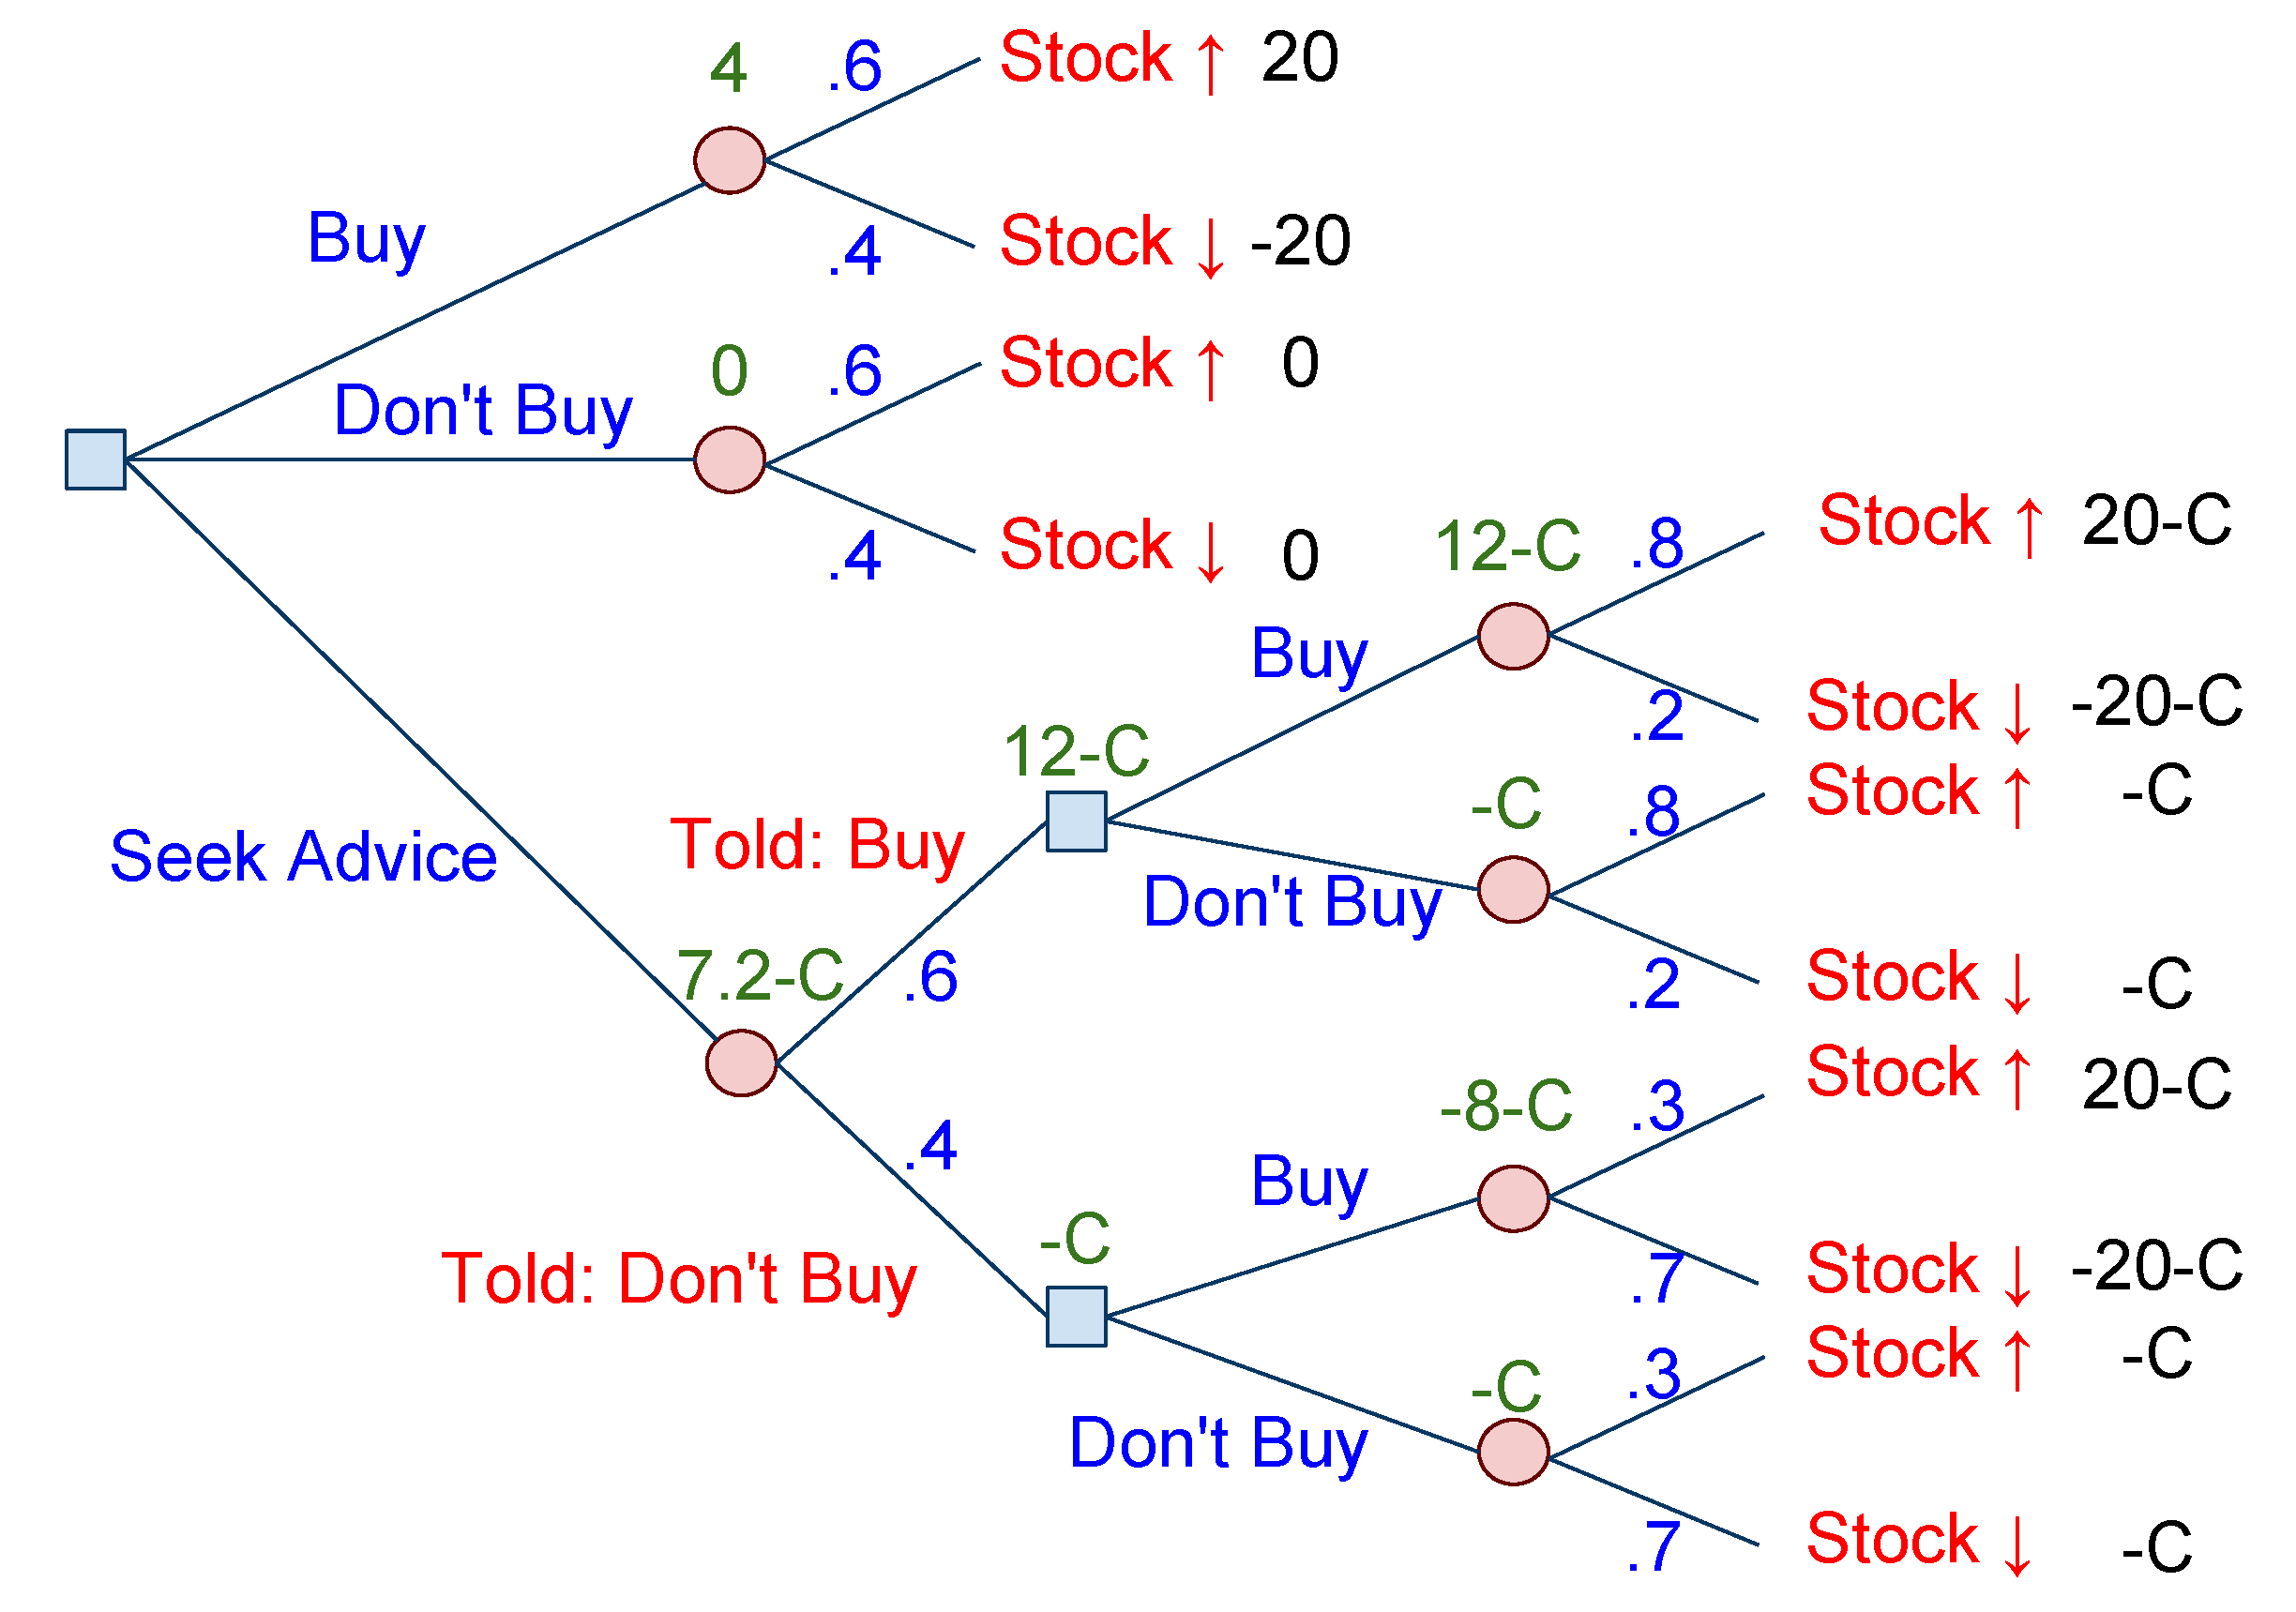
\includegraphics[width=10cm]{Stock_Example_Decision_Tree_11.pdf}
\end{center}


\end{document}
